\section{An Equivalence Graph Problem}


We can present a set of comparisons as a graph. Vertice are the coins, edges are the comparisons.


\begin{definition}
If comparing the edges of a graph results in at least one unbalanced edge in any condition.
We say this graph is a testing solution, feasible. Otherwise it's infeasible.
An optimal testing solution(denoted by $OTS$) is a solution with minimum number of edges(comparisons).
\end{definition}

An $OTS$ can presented by an integer partition as well, which is covered in Section 3.

\subsection*{Idea}
Consider a graph ${\cal G}(\pa,\pb)$ contains two disjoint cliques, one is $K_\pa$, another is $K_\pb$. The edges in ${\cal G}(\pa,\pb)$ means comparing the pair would results in balanced. Then we want to find a graph $g$ (number of vertices $\leq \pa+\pb$) which is not a subgraph of ${\cal G}(\pa,\pb)$.

\begin{lemma}
We can guarantee a graph $g$ (number of vertices $\leq \pa+\pb$) has a unbalanced edge iff $g$ is not a subgraph of ${\cal G}(\pa,\pb)$.
\end{lemma}

\begin{proof}

Denote the real coins as '+' and the fake ones as '$-$'. 

We compare edges of $g$. Vertices of $g$ are subset of vertices of ${\cal G}(\pa,\pb)$.
If $g$ is a subgraph of ${\cal G}(\pa,\pb)$, assign '+'s and '$-$'s from ${\cal G}$ to $g$ , $g$ results in all balance.
If it's not a subgraph of ${\cal G}(\pa,\pb)$, then at least one edge results in unbalance. We can prove this by contradiction. If $g$ results in all balance, edges in $g$ are either ('+','+') or ('$-$','$-$'), subset of edges of ${\cal G}(\pa,\pb)$, thus $g$ is a subgraph of ${\cal G}(\pa,\pb)$.
\end{proof}

\begin{figure}[H]
  \centering
  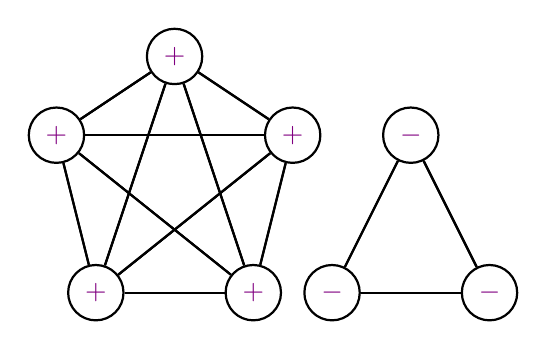
\begin{tikzpicture}[auto, thick]
\tikzstyle{vertex}=[draw,circle,text=violet,minimum width=20pt]
  \foreach \place/\name in {{(0,0)/a},
                            {(-0.5,2)/b},
                            {(2,0)/c},
                            {(2.5,2)/d},
                            {(1,3)/e}}
    \node[vertex] (\name) at \place {$+$};
  \foreach \place/\name in {{(3,0)/f},
                            {(5,0)/g},
                            {(4,2)/h}}
    \node[vertex] (\name) at \place {$-$};
  \foreach \source in {a,b,c,d,e}
    \foreach \dest in {a,b,c,d,e}
      \path (\source) edge (\dest);
  \foreach \source in {f,g,h}
    \foreach \dest in {f,g,h}
      \path (\source) edge (\dest);
\end{tikzpicture}
  \caption{${\cal G}(3,5)$}
\end{figure}

\begin{figure}[!htb]
  \minipage{0.3\textwidth}
    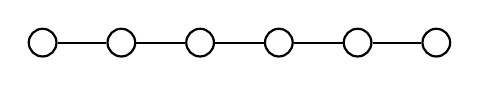
\begin{tikzpicture}[auto, thick]
\tikzstyle{vertex}=[draw,circle,text=violet,minimum width=10pt]
  \foreach \place/\name in {{(0,0)/a},
                            {(1,0)/b},
                            {(2,0)/c},
                            {(3,0)/d},
                            {(4,0)/e},
                            {(5,0)/f}}
    \node[vertex] (\name) at \place {};
  \foreach \source/\dest in {a/b,b/c,c/d,d/e,e/f}
      \path (\source) edge (\dest);
\end{tikzpicture}
    \caption{a trivial solution}
  \endminipage\hfill
  \minipage{0.3\textwidth}
    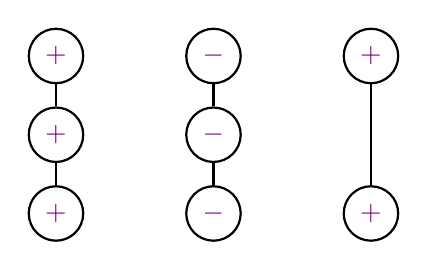
\begin{tikzpicture}[auto, thick]
\tikzstyle{vertex}=[draw,circle,text=violet,minimum width=15pt]
  \foreach \place/\name in {{(0,0)/a},
                            {(0,1)/b},
                            {(0,2)/c},
                            {(4,0)/g},
                            {(4,2)/h}}
    \node[vertex] (\name) at \place {$+$};
  \foreach \place/\name in {{(2,0)/d},
                            {(2,1)/e},
                            {(2,2)/f}}
    \node[vertex] (\name) at \place {$-$};
  \foreach \source/\dest in {a/b,b/c,d/e,e/f,g/h}
      \path (\source) edge (\dest);
\end{tikzpicture}
    \caption{not a solution since it's a subgraph of ${\cal G}(3,5)$, we can assign '+'s and '-'s as in the figure such that all edges are balanced.}
  \endminipage\hfill
  \minipage{0.3\textwidth}
    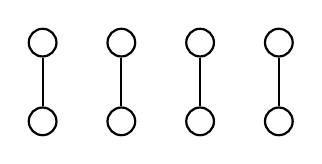
\begin{tikzpicture}[auto, thick]
\tikzstyle{vertex}=[draw,circle,text=violet,minimum width=10pt]
  \foreach \place/\name in {{(0,0)/a},
                            {(0,1)/b},
                            {(1,0)/c},
                            {(1,1)/d},
                            {(2,0)/e},
                            {(2,1)/f},
                            {(3,0)/g},
                            {(3,1)/h}}
    \node[vertex] (\name) at \place {};
  \foreach \source/\dest in {a/b,c/d,e/f,g/h}
      \path (\source) edge (\dest);
\end{tikzpicture}
    \caption{an optimal solution.}
  \endminipage
\end{figure}

Intuitively, if finding unbalance in a comparison, the game ends. But sometimes we can point a pair is unbalance after k comparisons(k is the answer) before the unbalance appears. The following shows $k_{min}=t_{min}-1$, which means the answer for Problem 4 is $t_{min}-1$

\begin{lemma}
$t_{min} = k_{min}+1 $
\end{lemma}

\begin{proof}
We divide the proof of the equation into two inequations

If we could point out a pair $e$ is unbalanced through the optimal graph $F$(with $k_{min}$ comparisons).
Consider a graph with these $k_{min}$ edges + $e$ which is not a subgraph of ${\cal G}(\pa,\pb)$
\[t_{min}\leq k_{min}+1\]

For a optimal graph $E$(with $t_{min}$ edges) which is not a subgraph of ${\cal G}(\pa,\pb)$. Let $E'$ = ($E$ remove an arbitrary edge $e$), then through $E'$. If $E'$ has unbalance comparison, we conclude the one is unbalanced, otherwise we could conclude $e$ is unbalanced.
Either case shows $E'$ is enough to end the game.
\[k_{min} \leq t_{min}-1\]

From the above inequations, the lemma holds.

\end{proof}

\subsection*{Goal}
We want to find a graph $g(\pa,\pb)$ that has minimum edges and $g(\pa,\pb)$ is not a subgraph of ${\cal G}(\pa,\pb)$. Through testing $g(\pa,\pb)-$an arbitrary edge $e$, we can point out a pair is unbalanced and it's optimal.

\begin{definition}
$\tau(\pa,\pb)$ is the number of edges of $OTS(\pa,\pb)$
\end{definition}

For example, $\tau(1,2)=2$, since testing a pair may result in balanced. On the other hand, testing two non-duplicate pair, one of them must results in unbalanced.

In this case, testing a pair is enough to point out a real coin and a fake one. 

Denote the coins we test as $coin_a$ $coin_b$ , the coin we didn't test as $coin_c$
If $coin_a$ and $coin_b$ is not balanced, then point out $coin_a$ and $coin_b$. Otherwise, point out $coin_a$ and $coin_c$

\begin{theorem}
Any graph with $n \leq \pa + \pb$ vertices and $m \leq \lfloor (\pa+\pb)/2 \rfloor-1$ edges $(0<\pa \leq \pb)$ 
is always a subgraph of ${\cal G}(\pa,\pb)$ (or equivalently, a subgraph of ${\cal G}(\pb,\pa)$).
\end{theorem}

\begin{proof}
We shall prove this theorem by induction.  \\

\noindent
{\bf (Basis Case:)} If $\pa = \pb =1$, then $\lfloor (\pa+\pb)/2 \rfloor-1 = 0$. Any graph with $n \leq 2$ vertices and $m \leq 0$ edges (i.e., no edges) is always a subgraph of ${\cal G}(1,1)$.
\\

\noindent
{\bf (Inductive Case:)} Suppose that the theorem holds for all $\pa + \pb \leq k$.  Our target is to show that the theorem also holds for the case $\pa + \pb = k + 1$ with $\pa \leq \pb$.   Consider a graph $G$ with  $n \leq k+1$ vertices and with $m \leq \lfloor (k+1)/2 \rfloor -1$ edges. 

\begin{enumerate}
  \item If $G$ is connected, then $n \leq m + 1 \leq (k+1)/2 \leq b$, which is a subgraph of $K_b$, 
           and thus a subgraph of ${\cal G}(\pa,\pb)$.   

  \item Otherwise, $G$ is not connected.  If $G$ has no edges, then $G$ is obviously a subgraph of ${\cal G}(\pa,\pb,0)$ 
          since $G$ has at most $\pa+\pb$ vertices.
          Else, let $C$ be the connected component of $G$ with the largest number $n'$ of vertices (so that $n' \geq 2$.
          Then, the number of edges in $C$ is at least $n'-1$.  To complete the proof, it is sufficient to show 
          that $G - C$ is a subgraph of ${\cal G}(\pa, \pb - n')$, as we can map $C$ as a subgraph in $K_b$.

The number of vertices in $G-C$ is $k+1-n' = \pa + (\pb-n')$, and the number of edges of $G-C$ is at most 
\begin{eqnarray*}
m - (n'-1) \leq \floor{(k+1)/2} - n' &=& \floor{(k+1)/2 - n'} \\
&=& \floor{ (k+1-n')/2 - n'/2 } \\
&\leq& \floor{ (k+1-n')/2 - 1 } \\
&=& \floor{(k+1-n')/2} - 1 = \floor{ (\pa + (\pb+n'))/2 } - 1.
\end{eqnarray*}
By induction hypothesis, $G-C$ is a subgraph of ${\cal G}(\pa, \pb-n')$, 
and consequently $G$ is a subgraph of ${\cal G}(\pa,\pb)$.
\end{enumerate}
In all cases, $G$ is a subgraph of ${\cal G}(\pa,\pb)$.  This completes the proof of the induction case, so that by the principle of mathematical induction, the theorem follows.
\end{proof}

\begin{corollary}
for all odd number $\pa,\pb$, $\tau(a,b)=\frac{\pa+\pb}{2}$
\end{corollary}

Consider a graph  $g(a,b)$ that have  $\frac{a+b}{2}$ components, each components have only two nodes. then  $g(\pa,\pb)$ is not a subgraph of  ${\cal G}(\pa,\pb)$, and by Thm2.2, it is the optimal solution.

\begin{theorem} 
For every $a,b$, we have a 2-approximation solution of  $\tau(\pa,\pb)$.
\end{theorem}
Consider a line with $max(\pa,\pb)$ nodes as in Figure 2. The graph is not a subgraph of  ${\cal G}(\pa,\pb)$, and by Thm2.2, it is a 2-approximation solution.
